%
%
%

\chapter{Introduction to Control Engineering with Python}

\section{Problem Statement and Learning Objectives}

This brief chapter will introduce
some control engineering computations with Python.  After completing this
chapter the student should be able to
\begin{itemize}
    \item Apply previous knowledge of Python basics to numerical evaluation of problems in this
    course.   We will use
    \begin{itemize}
            \item numpy, scipy, and matplotlib packages (python control references a package called Slycot but we do not need it.)
            \item python 3 (3.12 or later)  (command line or notebook environments)
            \item package python control (version 0.10+)
    \end{itemize}
    \item Write or adapt python scripts for control related computations including:
    \begin{itemize}
        \item enter a transfer function.
        \item Generate Bode and Root Locus Plots
        \item Correct the axis scales on plots to increase quality and readability of
        graphics plots.
        \item Use and adapt a supplied python package to optimize gains for PID control
        design in spite of actuator saturation and other non-ideal factors.
    \end{itemize}
\end{itemize}



\section{Links and details}
For download and detailed documentation, please see

\href{python control}{https://pypi.org/project/control/}

\href{Install Python on Windows}{https://learn.microsoft.com/en-us/windows/python/beginners}


\section{Root Locus Example}

Let's do the Root locus plot of Example 6.8.  The open loop gain is:
\beq\label{pythonRLsystem}
G(s) = C(s)P(s) = \frac {K(s+4)(s+5)} {(s+1+3j)(s+1-3j)}
\eeq

An example was simply generated by asking Claude.ai to plot the root locus of the above loop gain (input to Claude as LaTex code).

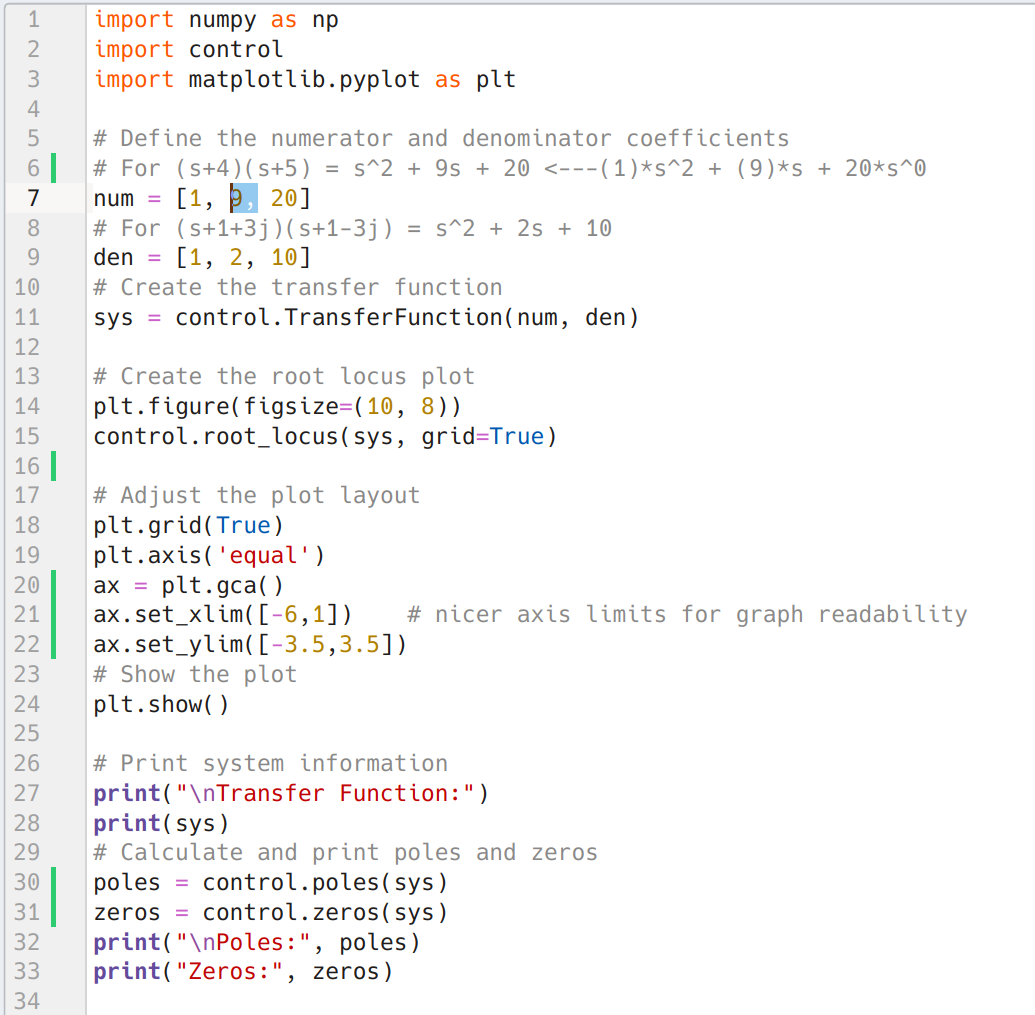
\includegraphics[width=0.35\textwidth]{figs08/python_rl_code_Chapt08.png}

In lines 7-9 the poles and zeros are multiplied out to form normalized polynomials in $s$, and
they are represented as a vector of the coefficients of the powers of $s$.  For example in the
numerator:
\[
(s+4)(s+5) = s^2 + 9s + 20 \to [1, 9, 20]
\]
we use the {\tt control.TransferFunction(num, den)}  call to make the numerator and denominator into
a {\tt TransferFunction()} object (line 11).

Then in lines 14 and 15, we open a figure in {\tt matplotlib} and use the {control.root\_locus()} method to plot it.

\begin{figure}
    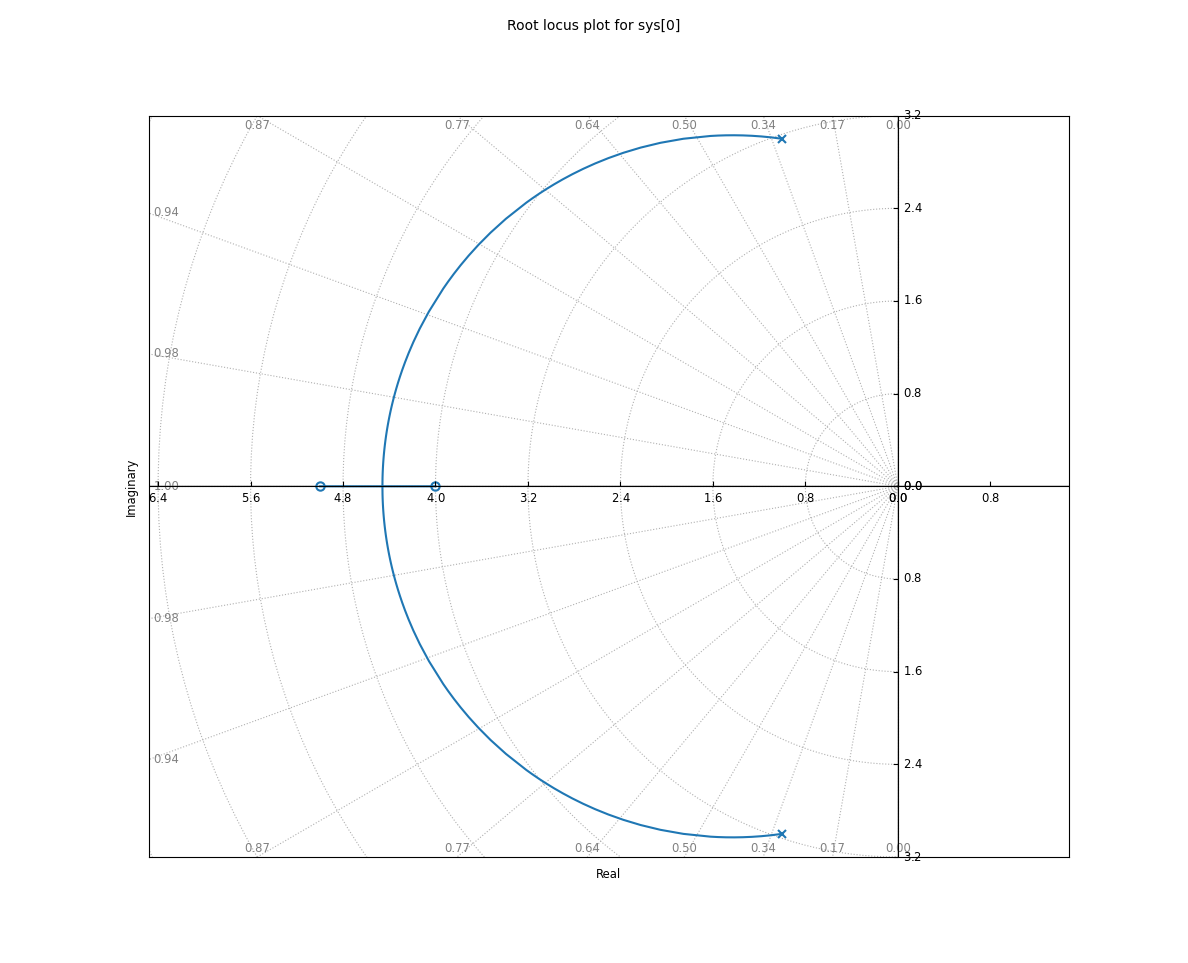
\includegraphics[width=\textwidth]{figs08/python_rl_result_Chapt08.png}
    \caption{Root locus of the system of Figure \ref{pythonRLsystem}.}\label{pythonRLoutput}
\end{figure}

\section{Plotting Ranges for high quality graphics}
Sometimes autoranges provided by graphing software do not result in a graph which shows the desired features.

The default ranges this time are OK but it feels like integer value axis limits would look better
so those are explicitly set in lines 21,22.

This is more important when you plot and compare multiple different root loci.   With autoranging,
all the plots can look the same until you read the axis limits which defeats the purpose of plotting.


% \section{Summary of Notation}

